\documentclass{article}\usepackage[]{graphicx}\usepackage[]{xcolor}
% maxwidth is the original width if it is less than linewidth
% otherwise use linewidth (to make sure the graphics do not exceed the margin)
\makeatletter
\def\maxwidth{ %
  \ifdim\Gin@nat@width>\linewidth
    \linewidth
  \else
    \Gin@nat@width
  \fi
}
\makeatother

\definecolor{fgcolor}{rgb}{0.345, 0.345, 0.345}
\newcommand{\hlnum}[1]{\textcolor[rgb]{0.686,0.059,0.569}{#1}}%
\newcommand{\hlstr}[1]{\textcolor[rgb]{0.192,0.494,0.8}{#1}}%
\newcommand{\hlcom}[1]{\textcolor[rgb]{0.678,0.584,0.686}{\textit{#1}}}%
\newcommand{\hlopt}[1]{\textcolor[rgb]{0,0,0}{#1}}%
\newcommand{\hlstd}[1]{\textcolor[rgb]{0.345,0.345,0.345}{#1}}%
\newcommand{\hlkwa}[1]{\textcolor[rgb]{0.161,0.373,0.58}{\textbf{#1}}}%
\newcommand{\hlkwb}[1]{\textcolor[rgb]{0.69,0.353,0.396}{#1}}%
\newcommand{\hlkwc}[1]{\textcolor[rgb]{0.333,0.667,0.333}{#1}}%
\newcommand{\hlkwd}[1]{\textcolor[rgb]{0.737,0.353,0.396}{\textbf{#1}}}%
\let\hlipl\hlkwb

\usepackage{framed}
\makeatletter
\newenvironment{kframe}{%
 \def\at@end@of@kframe{}%
 \ifinner\ifhmode%
  \def\at@end@of@kframe{\end{minipage}}%
  \begin{minipage}{\columnwidth}%
 \fi\fi%
 \def\FrameCommand##1{\hskip\@totalleftmargin \hskip-\fboxsep
 \colorbox{shadecolor}{##1}\hskip-\fboxsep
     % There is no \\@totalrightmargin, so:
     \hskip-\linewidth \hskip-\@totalleftmargin \hskip\columnwidth}%
 \MakeFramed {\advance\hsize-\width
   \@totalleftmargin\z@ \linewidth\hsize
   \@setminipage}}%
 {\par\unskip\endMakeFramed%
 \at@end@of@kframe}
\makeatother

\definecolor{shadecolor}{rgb}{.97, .97, .97}
\definecolor{messagecolor}{rgb}{0, 0, 0}
\definecolor{warningcolor}{rgb}{1, 0, 1}
\definecolor{errorcolor}{rgb}{1, 0, 0}
\newenvironment{knitrout}{}{} % an empty environment to be redefined in TeX

\usepackage{alltt}
\usepackage[utf8]{inputenc}
\usepackage{amsfonts}
\usepackage{tgpagella}
\usepackage{graphicx} % Required for inserting images
\usepackage{polski}
\renewcommand*{\figurename}{Rysunek}
\usepackage{nicefrac, xfrac}
\usepackage[margin=1in]{geometry}
\usepackage{hyperref}
\usepackage{xcolor}
\usepackage{amssymb}
\usepackage[bottom]{footmisc}
\usepackage{float}
\IfFileExists{upquote.sty}{\usepackage{upquote}}{}
\begin{document}



\section{Liczba naprawianych pojazdów w każdym miesiącu pracy warsztatu}

\begin{knitrout}
\definecolor{shadecolor}{rgb}{0.969, 0.969, 0.969}\color{fgcolor}\begin{figure}[H]

{\centering 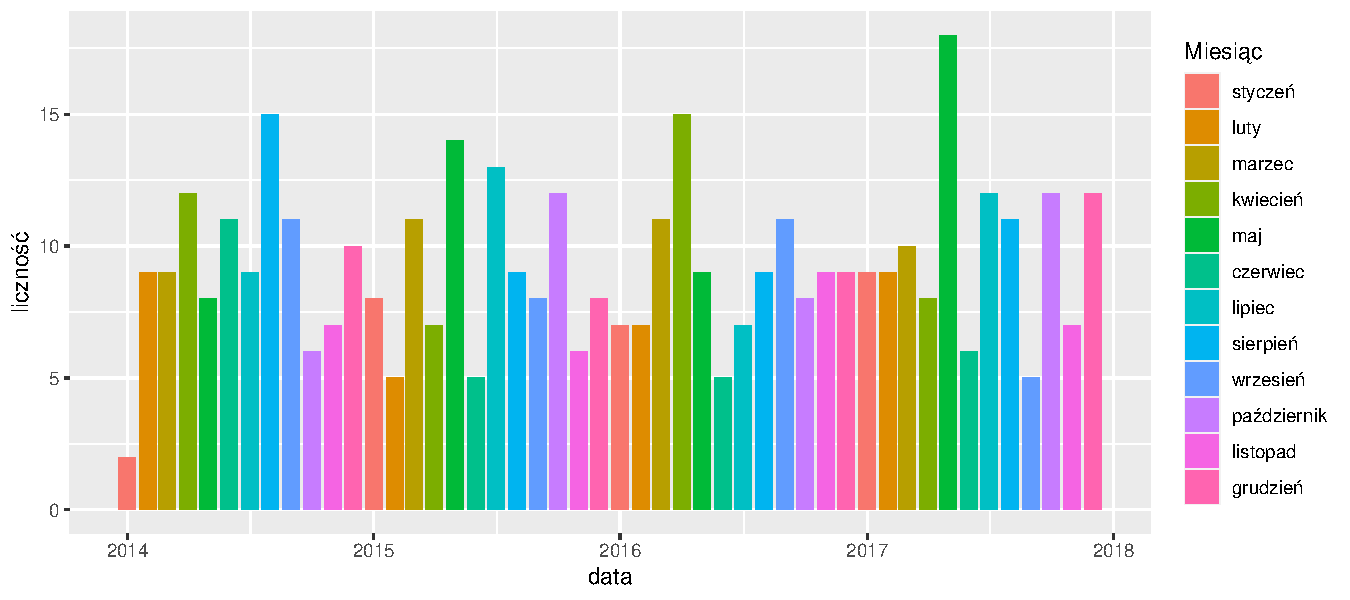
\includegraphics[width=\maxwidth]{figure/fig_naprawy_miesiecznie-1} 

}

\caption[Wykres liczba naprawianych pojazdów w każdym miesiącu pracy warsztatu]{Wykres liczba naprawianych pojazdów w każdym miesiącu pracy warsztatu}\label{fig:fig_naprawy_miesiecznie}
\end{figure}

\end{knitrout}

Wykres \ref{fig:fig_naprawy_miesiecznie} przedstawia liczbę naprawionych pojazdów w każdym miesiącu pracy warsztatu. Najwięcej pojazdów zostało naprawionych w miesiącach: 
maj 2017,
a było ich 18. Natomiast najmniej przeprowadzonych napraw było w miesiącach:
styczeń 2014,
było ich 2. Średnia liczba napraw miesięcznie wynosi 
9.188. 

\section{Tabela najlepszych okazji}

Zostanie teraz omówiona tabela najlepszych okazji, czyli pojazdów skupionych i sprzedanych, które przyniosły najwięcej zysku. Został uwzględniony także koszt naprawy pojazdu, gdy była ona potrzebna.





\begin{knitrout}
\definecolor{shadecolor}{rgb}{0.969, 0.969, 0.969}\color{fgcolor}\begin{kframe}
\begin{verbatim}
##     id_samochodu         marka    model   zysk
## 636          742 Mercedes-Benz E 63 AMG 126558
## 497          592       Porsche Panamera  99182
## 175          221 Mercedes-Benz    E 300  98044
## 805          779        Jaguar      XKR  87200
## 881          969       Porsche Panamera  82355
\end{verbatim}
\end{kframe}
\end{knitrout}

Największy zysk ze sprzedaży pojazdu warsztat odniósł dla pojazdu o id 742. Jest nim Mercedes-Benz o modelu E 63 AMG. Warsztat zarobił on na nim około 126.56 tys. zł. 
Na drugim miejscu znajduje się Porsche o modelu Panamera. Zysk z tego pojazdu wyniósł około 99.18 tys. zł, czyli o około 27.38 tys. zł mniej niż dla pojazdu znajdującego się na pierwszym miejscu, czyli różnica w cenie jest duża.
W trzeciej kolejności najwięcej zarobił pojazd Mercedes-Benz o modelu E 300, na którym warsztat zarobił około 98.04 tys. zł. Jest to mniej od poprzedniego pojazdu o około 1.14 tys. zł, czyli różnica w cenie jest niewielka. 
Ogólnie każdy pojazd znajdujący się w top 5 najlepszych okazji przyniósł zysk wielkości przynajmnej 80 tyś. zł.

\section{Profil klienta}

W następnej kolejności zostaną przeanalizawani klienci warsztatu. Zostaną sprawdzone liczności klientów ze względu na różne ich cechy.

\subsection{Płeć}

Pierwszą cechą wziętą pod uwagę jest płeć klienta. Zostanie sprawdzone, ile jest kobiet i mężczyzn wśród naszych klientów oraz jak duża jest różnica w licznościach tych grup.

\begin{knitrout}
\definecolor{shadecolor}{rgb}{0.969, 0.969, 0.969}\color{fgcolor}\begin{figure}[H]

{\centering 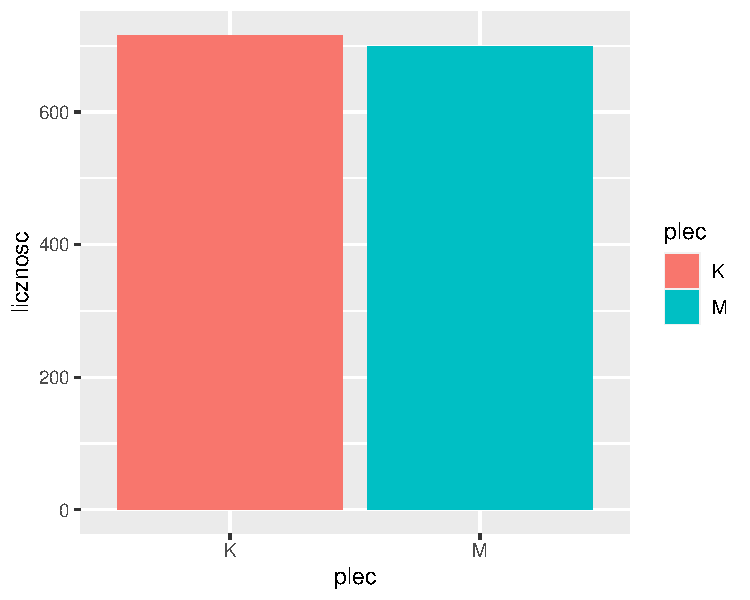
\includegraphics[width=\maxwidth]{figure/fig_plec-1} 

}

\caption[Wykres liczby klientów przy podziale ze względu na płeć]{Wykres liczby klientów przy podziale ze względu na płeć}\label{fig:fig_plec}
\end{figure}

\end{knitrout}

Na wykresie słupkowym \ref{fig:fig_plec} są zaprezentowane liczności klientów przy podziale ze względu na płeć. Więcej klientów warsztatu należy do grupy kobiet, jest ich 714. Grupa kobiet jest około 1.102
razy większa od grupy mężczyzn (jest ich 648), a zatem różnica jest nieduża.

\subsection{Wiek}

Zostanie również przeanalizowany rozkład wieku klientów warsztatu.





\begin{knitrout}
\definecolor{shadecolor}{rgb}{0.969, 0.969, 0.969}\color{fgcolor}\begin{figure}[H]

{\centering 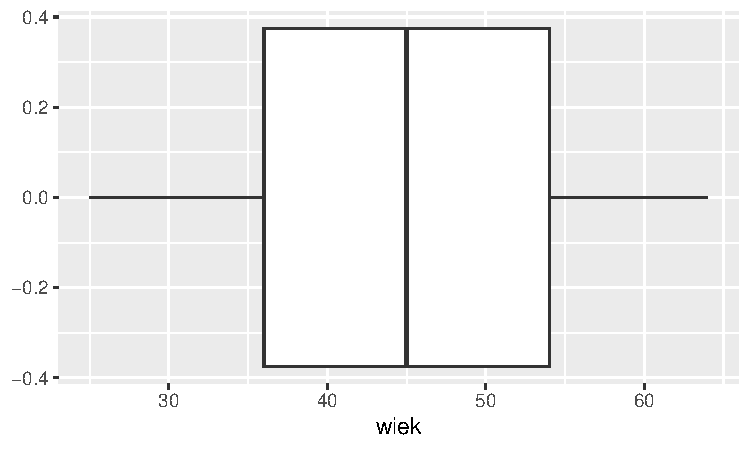
\includegraphics[width=\maxwidth]{figure/fig_wiek-1} 

}

\caption[Wykres pudełkowy wieku klientów]{Wykres pudełkowy wieku klientów}\label{fig:fig_wiek}
\end{figure}

\end{knitrout}

Rysunek \ref{fig:fig_wiek} przedstawia wykres pudełkowy wieku klientów warsztatu. Widać, że mediana wieku wynosi 45 lat, natomiast pierwszy kwartyl wynosi 36 lat, trzeci kwartyl natomiast 54 lata. Zatem połowa klientów warsztatu jest wieku między 36 lat a 54 lata.
Najmłodszy klient warsztatu ma 25 lat, natomiast najstarszy jest w wieku 64 lat.



\begin{table}[H]
\centering
\begin{tabular}{c|c} \hline
Miara & Wartość \\ \hline
Średnia & 45.17 \\ 
Odchylenie standardowe & 10.73 \\
Skośność & 0.02  \\ 
Kurtoza & 1.86 \\ \hline
\end{tabular}
\caption{Wybrane miary wieku klientów}
\label{tab_wiek}
\end{table}

Kilka miar, których nie da się odczytać z wykresu pudełkowego, zostało przedstawionych w tabeli \ref{tab_wiek}. Można zatem odczytać, że średnio klieci mają 45.17 lat, a odchylenie standardowe wieku wynosi 10.73 lata. Wartość współczynnika skośności jest bliska 0, a zatem rozkład wieku można uznać za symetryczny. Kurtoza przyjmuje wartość większą od 0, a zatem rozkład wieku jest leptokurtyczny, czyli jest bardziej wysmukły niż normalny.

\subsection{Miasto}
\begin{knitrout}
\definecolor{shadecolor}{rgb}{0.969, 0.969, 0.969}\color{fgcolor}\begin{kframe}
\begin{verbatim}
##   miejsce       miasto liczność
## 1     1.0      Wrocław      708
## 2     2.0    Bydgoszcz       22
## 3     3.0         Łódź       20
## 4     5.5        Opole       16
## 5     5.5       Gdańsk       16
## 6     5.5 Zielona Góra       16
## 7     5.5       Poznań       16
\end{verbatim}
\end{kframe}
\end{knitrout}

Najwięcej klientów warsztatu pochodzi z miasta Wrocław. Liczniść w nim wynosi 708 klientów. W następnej kolejności najwięcej klientów pochodzi z miasta Bydgoszcz, z czego liczność w nim wynosi 22 klientów, czyli jest ich 32.18 mniej niż klientów z miasta Wrocław. Na miejscu 3 jest miasto Łódź, mieszka w nim 20 klientów. Natomiast na ostatnim miejscu przedstawionym w tabeli są miasta Opole, Gdańsk, Zielona Góra, Poznań, mieszka w nich 16 klientów.

\subsection{Karta lojalnościowa}

W tej części zostanie sprawdzone, ilu klientów posiada kartę lojalnościową. Klient zdobywa ją po skorzystaniu z usług warsztatu (naprawa, zakup lub sprzedaż pojazdu) przynajmniej trzy razy. Klient posiadający tę katrę może kupować samochody ze zniżką w wysokości 3\%.

\begin{knitrout}
\definecolor{shadecolor}{rgb}{0.969, 0.969, 0.969}\color{fgcolor}\begin{figure}[H]

{\centering 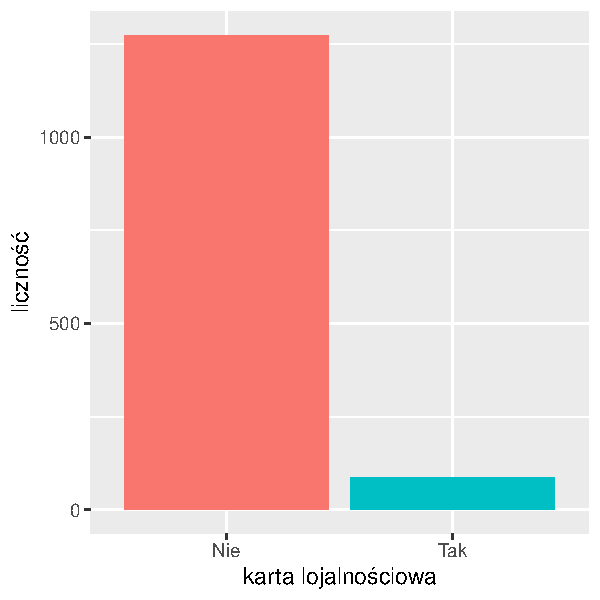
\includegraphics[width=\maxwidth]{figure/fig_karta-1} 

}

\caption[Wykres liczby klientów ze względu na posiadanie karty lojalnościowej]{Wykres liczby klientów ze względu na posiadanie karty lojalnościowej}\label{fig:fig_karta}
\end{figure}

\end{knitrout}

Bardzej liczną grupą są klienci, którzy nie posiadają karty lojalnoścowej, jest ich 1274 (94\% wszystkich klientów). W grupie klientów, którzy posiadają kartę lojalnoścową, jest 88 osób i stanowią oni 6\% klientów warsztatu.

\section{Jak wybrane cechy pojazdów wpływają na zysk warsztatu?}

W tym paragrafie zostaną opisane zależności między zyskiem ze sprzedaży pojazdów, skupionych i w razie potrzeby naprawionych przez warsztat, a cechami: rodzaj pojazdu, czy jest powypadkowy i pojemność silnika.

\subsection{Rodzaj pojazdu}

Pierwszą cechą braną pod uwagę jest rodzaj pojazdu, czyli czy jest to samochód czy motocykl.

\begin{knitrout}
\definecolor{shadecolor}{rgb}{0.969, 0.969, 0.969}\color{fgcolor}\begin{figure}[H]

{\centering 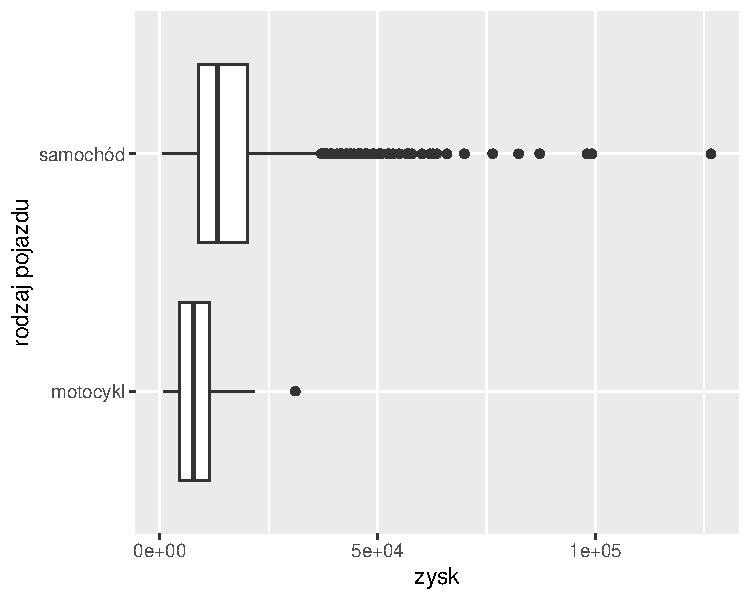
\includegraphics[width=\maxwidth]{figure/fig_typ-1} 

}

\caption[Wykresy pudełkowe zysku ze względu na rodzaj pojazdu]{Wykresy pudełkowe zysku ze względu na rodzaj pojazdu}\label{fig:fig_typ}
\end{figure}

\end{knitrout}

Na rysunku \ref{fig:fig_typ} przedstawione są dwa wykresy pudełkowe zysków, jeden dla samochodów, drugi dla motocykli. Większa mediana, wynosząca 13.332 tyś. zł, jest dla pojazdów typu samochód. W drugiej grupie wynosi ona 7.8 tyś. zł. 
Większy pierwszy kwartyl występuje w grupie typu samochód, wynosi on 8.896 tyś. zł, w porównaniu dla grupy typu motocykl jego wartość wynosi 4.488 tyś. zł.
W przypadku kwartyla trzeciego większa wartość występuje w grupie typu samochód (wynosi 20.164 tyś. zł). W drugiej grupie wynosi on 11.5 tyś. zł.
Największy zysk przyniósł samochód, a wyniósł on 126.558 tyś. zł. 
Najmniejszy zysk natomiast przyniósł samochód i wyniósł on 0.72 tyś. zł. Zatem częściej większy zysk dla warsztatu przynosi sprzedaż pojazdów typu samochód. 

\subsection{Czy powypadkowy}

Następną badaną cechą jest to, czy pojazd jest powypadkowy.

\begin{knitrout}
\definecolor{shadecolor}{rgb}{0.969, 0.969, 0.969}\color{fgcolor}\begin{figure}[H]

{\centering 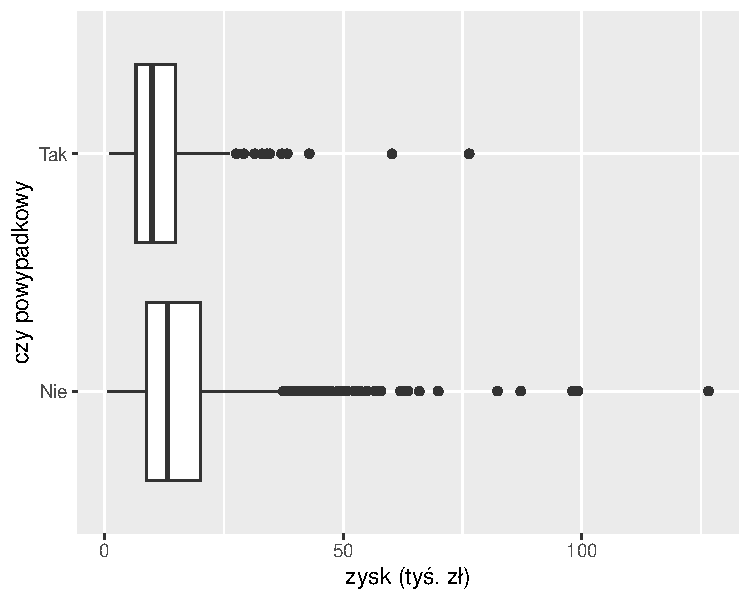
\includegraphics[width=\maxwidth]{figure/fig_wypadkowy-1} 

}

\caption[Wykresy pudełkowe zysku ze względu na to czy pojazd jest powypadkowy]{Wykresy pudełkowe zysku ze względu na to czy pojazd jest powypadkowy}\label{fig:fig_wypadkowy}
\end{figure}

\end{knitrout}

Na rysunku \ref{fig:fig_wypadkowy} przedstawione są dwa wykresy pudełkowe zysków dla pojazdów powypadkowych i niepowypadkowych. Większa mediana, wynosząca 13.206 tyś. zł, jest dla pojazdów niepowypadkowych. W drugiej grupie wynosi ona 9.908 tyś. zł. 
Większy pierwszy kwartyl występuje w grupie pojazdów niepowypadkowych, wynosi on 8.83 tyś. zł, w porównaniu dla grupy pojazdów powypadkowych jego wartość wynosi 6.58725 tyś. zł.
Większa wartość trzeciego kwartylu występuje dla pojazdów niepowypadkowych i wynosi 20.154 tyś. zł. Dla pojazdów powypadkowych wynosi on 14.954 tyś. zł.
Największy zysk przyniósł pojazd z grupy niepowypadkowych i wyniósł on 126.558 tyś. zł. 
Najmniejszy zysk natomiast przyniósł pojazd z grupy niepowypadkowych i wyniósł on 0.72 tyś. zł. Zatem częściej większy zysk dla warsztatu przynosi sprzedaż pojazdów niepowypadkowych. 

\subsection{Pojemność silnika}

Ostatnią cechą braną pod uwagę jest pojemność silnika pojazdu.

\begin{knitrout}
\definecolor{shadecolor}{rgb}{0.969, 0.969, 0.969}\color{fgcolor}\begin{figure}[H]

{\centering 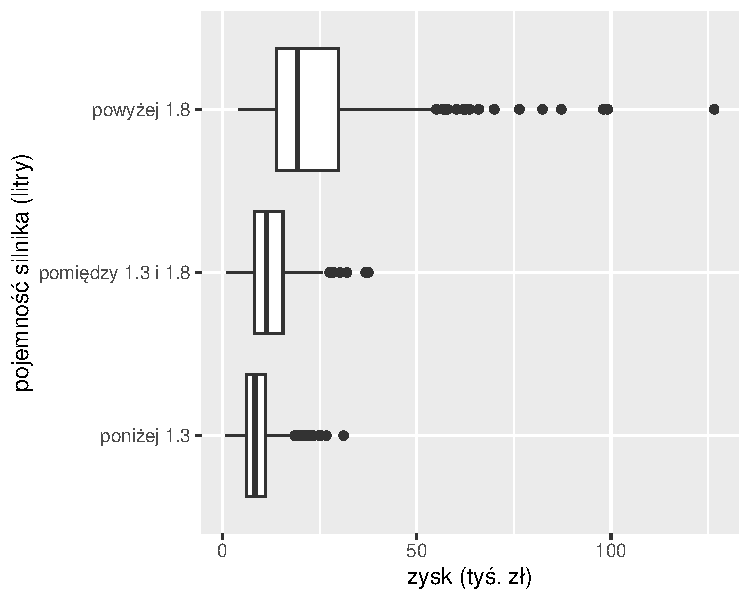
\includegraphics[width=\maxwidth]{figure/fig_pojemnosc-1} 

}

\caption[Wykresy pudełkowe zysku ze względu na pojemność silnika]{Wykresy pudełkowe zysku ze względu na pojemność silnika}\label{fig:fig_pojemnosc}
\end{figure}

\end{knitrout}

Na rysunku \ref{fig:fig_wypadkowy} przedstawione są wykresy pudełkowe zysków ze względu na pojemność silnika. Największa mediana, wynosząca 19.293 tyś. zł, jest dla pojazdów o pojemności silnika powyżej 1.8 litra. Natomiast najmniej ona wynosi 8.347 tyś. zł w grupie pojazdów o pojemności poniżej 1.3 litra. 
Największy pierwszy kwartyl występuje w grupie pojazdów o pojemności powyżej 1.8 litra, wynosi on 13.9385 tyś. zł, w porównaniu z pojazdami o pojemności poniżej 1.3 litra, dla których jego wartość jest najmniejsza i wynosi 6.19725 tyś. zł.
Największa wartość trzeciego kwartylu występuje dla pojazdów o pojemności powyżej 1.8 litra i wynosi 29.845 tyś. zł. Dla pojazdów poniżej 1.3 litra wynosi on 11.076 tyś. zł i jest to najmnijesza wartość w tych grupach.
Największy zysk przyniósł pojazd o pojemności silnika powyżej 1.8 litra i wyniósł on 126.558 tyś. zł. 
Najmniejszy zysk natomiast przyniósł pojazd z pojemnością silnika poniżej 1.3 litra i wyniósł on 0.72 tyś. zł. Zatem przeważnie największy zysk dla warsztatu przynosi sprzedaż pojazdów o pojemności silnika powyżej 1.8 litra. Najczęściej najmniejszy zysk przynosi sprzedaż pojazdów z pojemnością silnika poniżej 1.3 litra.

\section{Od tego miejsca bierz Martyna}

\section{Analiza bilansu}

\subsection{Analiza wydatków na zakup pojazdów}

Sprawdziliśmy, jak wyglądają miesięczne wydatki na zakup pojazdów, które w razie potrzeby warsztat naprawia, a następnie sprzedaje.

\begin{knitrout}
\definecolor{shadecolor}{rgb}{0.969, 0.969, 0.969}\color{fgcolor}\begin{figure}[H]

{\centering 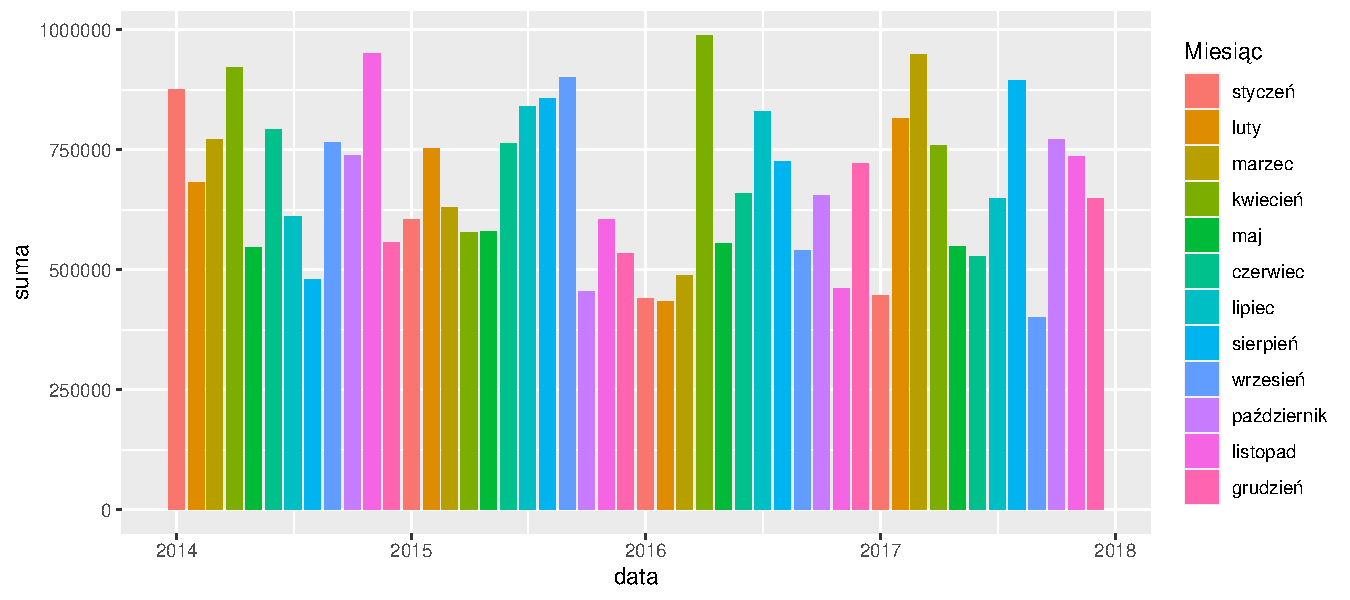
\includegraphics[width=\maxwidth]{figure/fig_zakup_pojazdu-1} 

}

\caption[Miesięczne wydatki na zakup pojazdów]{Miesięczne wydatki na zakup pojazdów}\label{fig:fig_zakup_pojazdu}
\end{figure}

\end{knitrout}

Wykres \ref{fig:fig_zakup_pojazdu} przedstawia miesięczne wydatki na zakup pojazdów. 
Największe wydatki warsztat miał w miesiącu kwiecień 2016. Były one w wysokości 989 tyś. zł. 
Wydatki wielkości 950.8 tyś. zł były drugimi najwyższymi i były 1.04 razy mniejsze od tych największych. Wystąpiły one w miesiącu listopad 2014.
Najmniejsze wydatki warsztat zaobserwował w miesiącu wrzesień 2017 i wyniosły one 400.3 tyś. zł. 
Drugie co do wielkości najniższe wydatki na zakup pojazdów wystąpiły miesiącu luty 2016, a wyniosły one 433.9 tyś. zł.
W każdym miesiącu działania warsztatu wydatki na zakup pojazdów wyniosły przynajmnej 400 tyś. zł.

\subsection{Analiza wydatków na zakup części}

Następnie zostało sprawdzone, jak wyglądają miesięczne wydatki na zakup części potrzebnych do napraw pojazdów.

\begin{knitrout}
\definecolor{shadecolor}{rgb}{0.969, 0.969, 0.969}\color{fgcolor}\begin{figure}[H]

{\centering 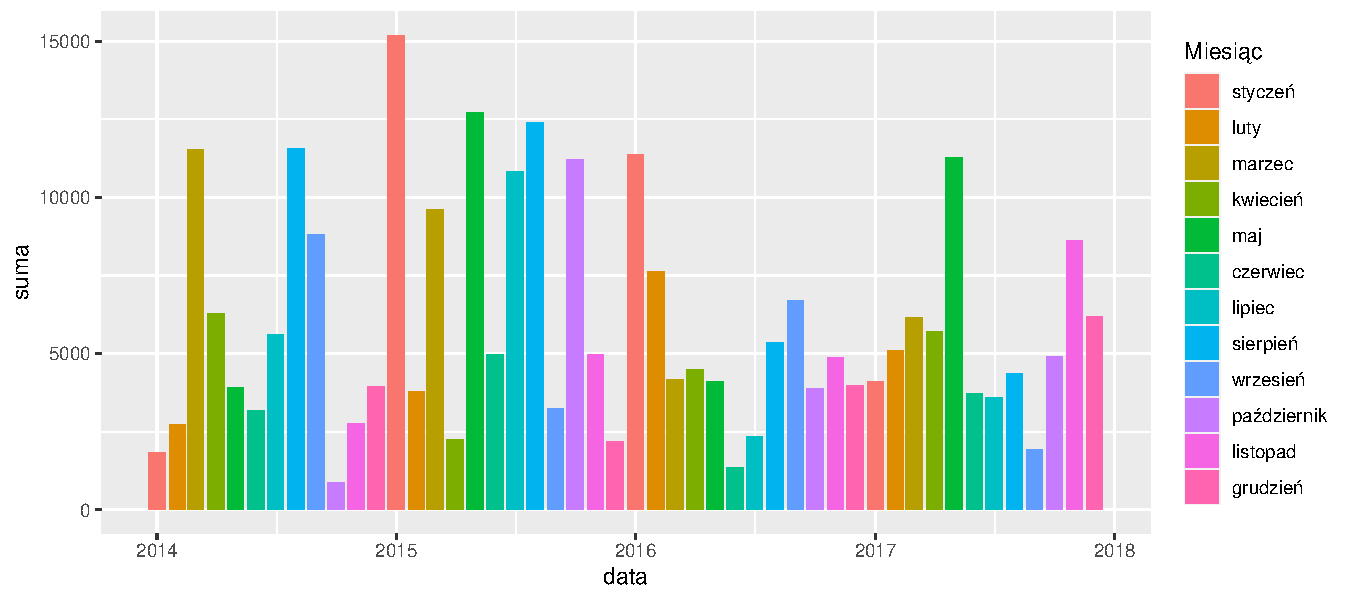
\includegraphics[width=\maxwidth]{figure/fig_zakup_czesci-1} 

}

\caption[Miesięczne wydatki na zakup części]{Miesięczne wydatki na zakup części}\label{fig:fig_zakup_czesci}
\end{figure}

\end{knitrout}

Wykres \ref{fig:fig_zakup_czesci} przedstawia miesięczne wydatki na zakup części do naprawy pojazdów.
Największe wydatki warsztat miał w miesiącu styczeń 2015 i wyniosły one 15.2 tyś. zł. 
Drugie najwyższye wydatkami były wielkości 12.73 tyś. zł i były 1.19 razy mniejsze od tych największych. Wystąpiły one w miesiącu maj 2015.
Najmniejsze wydatki na części zostały odnotowane w miesiącu październik 2014 i wyniosły 0.87 tyś. zł. 
Drugie najmniejsze wydatki wyniosły 1.37 tyś. zł. Wystąpił on w miesiącu czerwiec 2016.
Ogólnie w każdym miesiącu działania warsztatu wydatki na zakup części wyniosły przynajmnej 0.9 tyś. zł.

\subsection{Analiza przychodów z usług warsztatu}

Chcielibyśmy sprawdzić, jak wyglądają miesięczne przychody (lub straty) wynikające z prowadzenia warsztatu. Przez przychód za pojedyńczą usługę uważamy różnicę ceny, którą zapłacił klient i kwoty zapłaconej za części. Przeanaliowane zostaną przychody z uwzględnieniem kosztu własnych napraw oraz bez nich.

\begin{knitrout}
\definecolor{shadecolor}{rgb}{0.969, 0.969, 0.969}\color{fgcolor}\begin{figure}[H]

{\centering 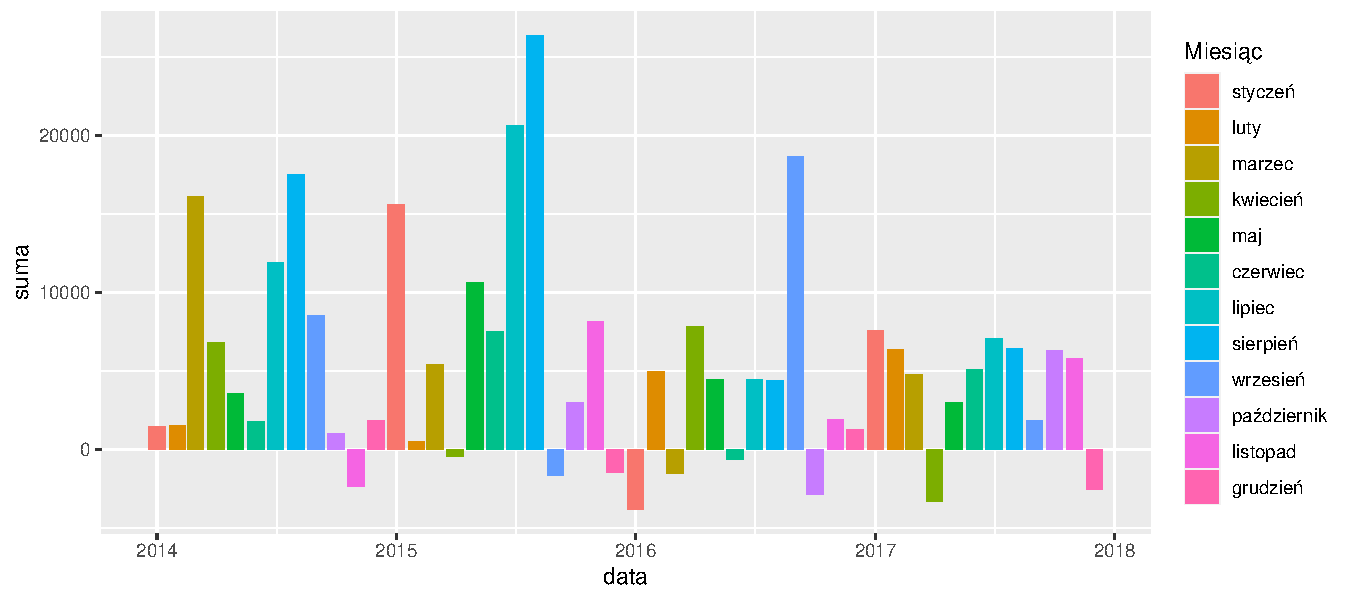
\includegraphics[width=\maxwidth]{figure/fig_uslugi-1} 

}

\caption[Miesięczny przychód wynikający z prowadzenia warsztatu z wliczonymi kosztami napraw własnych]{Miesięczny przychód wynikający z prowadzenia warsztatu z wliczonymi kosztami napraw własnych}\label{fig:fig_uslugi}
\end{figure}

\end{knitrout}

Na wykresie \ref{fig:fig_uslugi} przedstawiony jest miesięczny przychód wynikający z prowadzenia warsztatu. Zostały na nim uwzględnione koszty napraw własnych. 
Największy przychód był zaobserwowany w miesiącu sierpień 2015 i wyniósł on wtedy 26.37 tyś. zł.
Następny co do wielkości przychód wystąpił w miesiącu lipiec 2015, wyniósł on 20.61 tyś. zł. Jest on 1.28 razy mniejszy niż najwyższy przychód.
Najmniejszy przychód warsztat odnotował w miesiącu styczeń 2016, który wyniósł -3.86 tyś. zł. 
Drugi najmniejszy przychód wyniósł -3.34 tyś. zł i wystąpił w miesiącu kwiecień 2017.

\begin{knitrout}
\definecolor{shadecolor}{rgb}{0.969, 0.969, 0.969}\color{fgcolor}\begin{figure}[H]

{\centering 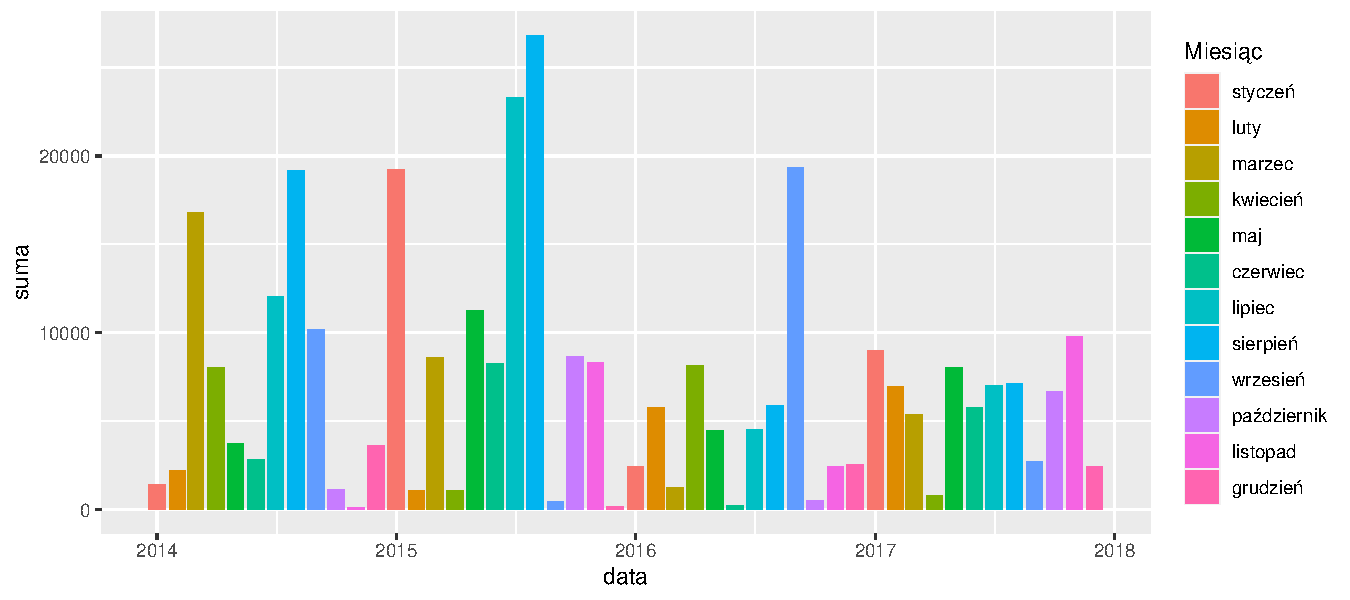
\includegraphics[width=\maxwidth]{figure/fig_uslugi2-1} 

}

\caption[Miesięczny przychód wynikający z prowadzenia warsztatu bez wliczonych kosztów napraw własnych]{Miesięczny przychód wynikający z prowadzenia warsztatu bez wliczonych kosztów napraw własnych}\label{fig:fig_uslugi2}
\end{figure}

\end{knitrout}

Na wykresie \ref{fig:fig_uslugi2} przedstawiony jest miesięczny przychód wynikający z prowadzenia warsztatu, ale tym razem bez uwzględnienia kosztów własnych. 
Największy przychód warsztat zaobserwował w miesiącu sierpień 2015, który wyniósł 26.83 tyś. zł.
Drugi zaś co do wielkości przychód wsytąpił w miesiącu lipiec 2015, wyniósł on 23.29 tyś. zł, czyli jest 1.15 razy mniejszy niż ten najwyższy zaobserwowany.
Najmniejszy przychód został odnotowany w miesiącu listopad 2014 i wyniósł 0.15 tyś. zł. 
Drugi najmniejszy przychód wyniósł 0.21 tyś. zł. Wystąpił on w miesiącu grudzień 2015.




\end{document}
